\documentclass{article}
\usepackage{graphicx}
\usepackage{pdfpages}

\begin{document}

{\large
    DELETE THE FOLLOWING MESSAGE WHEN COMPLETED
}
\\  
    THIS SECTION OF D4 ONLY HAS INTO ACCOUNT THE FOLLOWING VARIABLES:
    \begin{itemize}
        \item Education
        \item MaritalSts
        \item Income 
        \item Kidhome
        \item Teenhome
        \item Recency
        \item Response
        \item Complain
        \item Age
    \end{itemize}


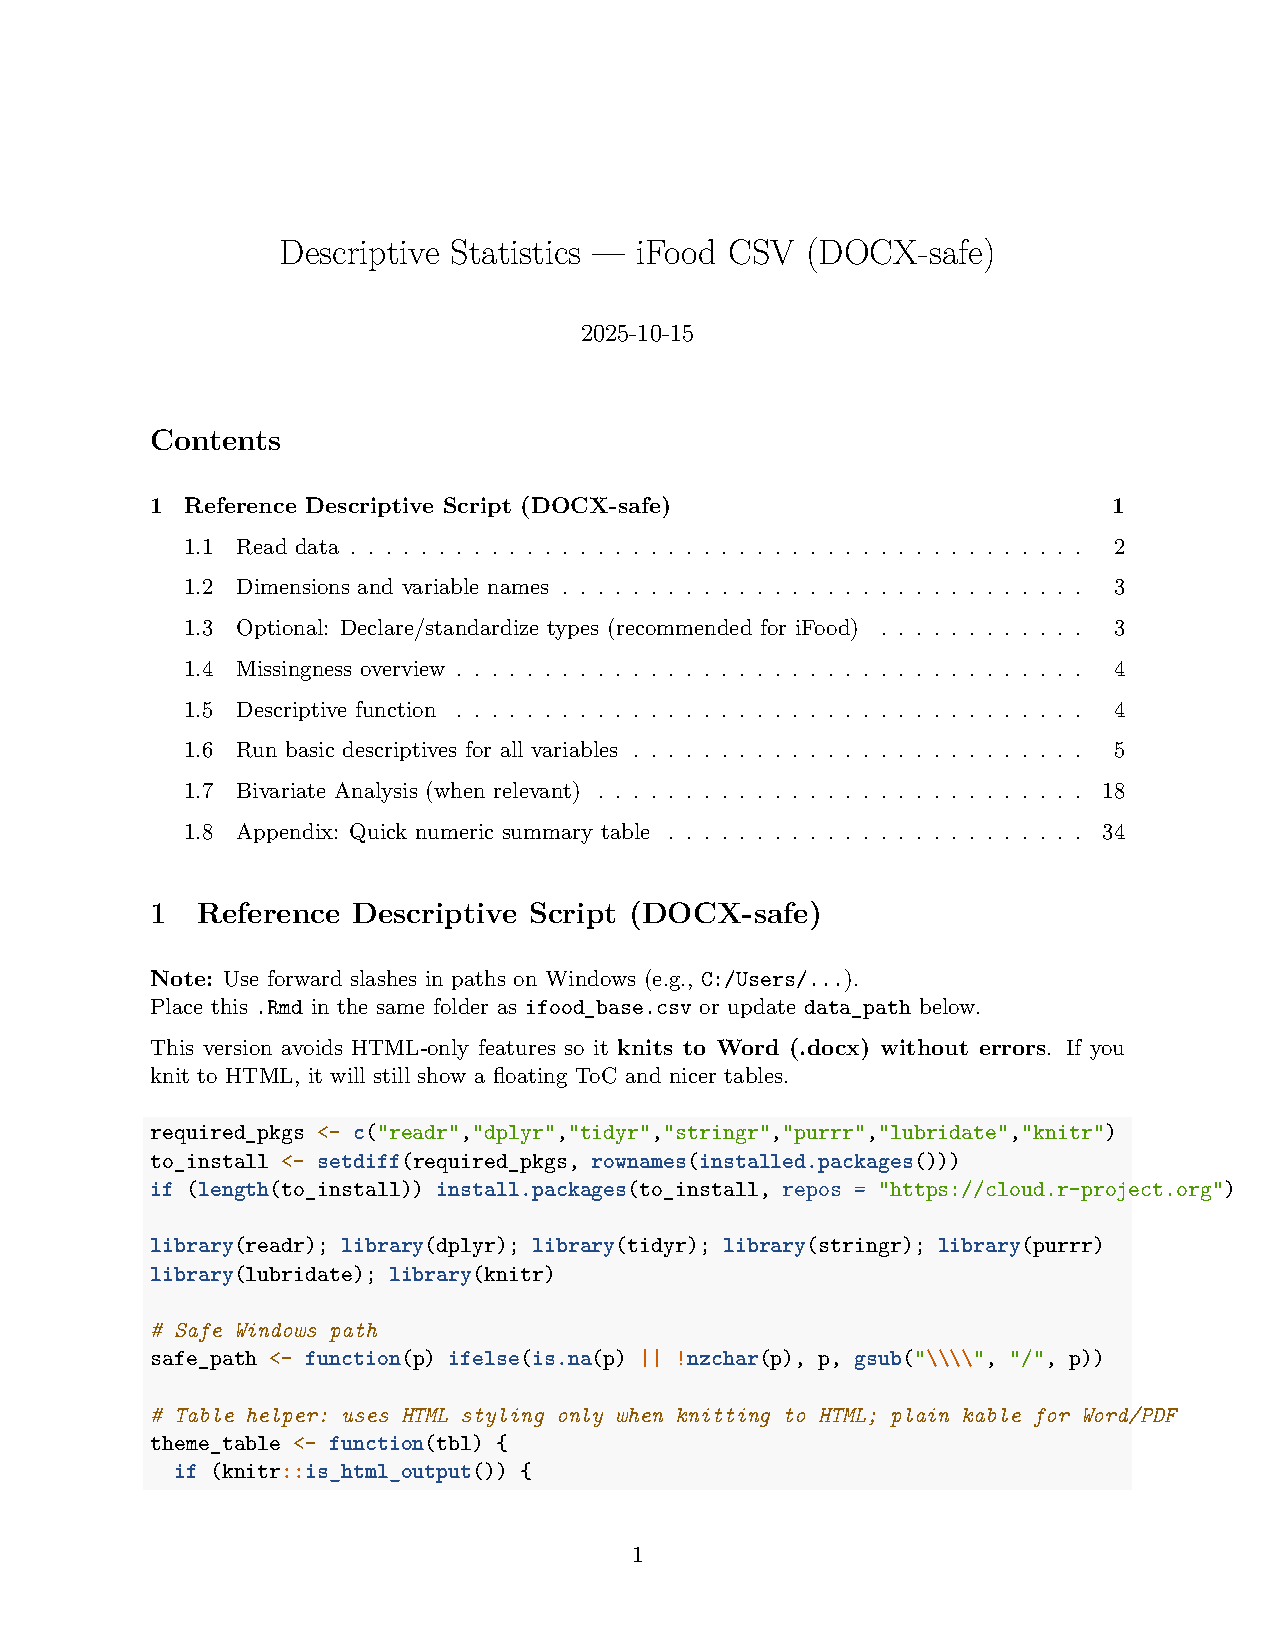
\includepdf[pages=-, scale=0.8, pagecommand={}, fitpaper=true]{Descriptive Statistics}


\paragraph{{Final data description}}

The iFood dataset includes 2,031 customers across nine variables, showing no missing data and excellent quality. Customers are predominantly middle-aged and well-educated, with a wide but reasonable income range (mean €52,844). Family structures are typically small, and complaints are extremely rare (0.98\%). Income relates positively to education and age but negatively to having children, while higher-income, recently active customers respond more to marketing campaigns. Overall, the data are well-behaved, balanced across variables, and suitable for multivariate modeling, with only one extreme income outlier and an imbalanced “Complain” variable as minor considerations.

\end{document}
